% chercher des documents LaTeX dans styles, corps et bib
\makeatletter\def\input@path{{styles/}{body/}{bib/}}\makeatother

% Utiliser le style rapport.cls
\documentclass[a4paper]{article}

\usepackage[a4paper,vdivide={*,22cm,4cm}]{geometry}
%\usepackage[french]{babel} % style francais
\usepackage{pageGardeEnsta}
\usepackage{lmodern}
\usepackage[T1]{fontenc}
\usepackage[utf8]{inputenc}
\usepackage{indentfirst}

%============ insert code into latex ==============
\usepackage{listings}
\usepackage{color}

\definecolor{dkgreen}{rgb}{0,0.6,0}
\definecolor{gray}{rgb}{0.5,0.5,0.5}
\definecolor{mauve}{rgb}{0.58,0,0.82}

\lstset{frame=tb,
  language=Ruby,
  aboveskip=3mm,
  belowskip=3mm,
  showstringspaces=false,
  columns=flexible,
  basicstyle={\small\ttfamily},
  numbers=none,
  numberstyle=\tiny\color{gray},
  keywordstyle=\color{blue},
  commentstyle=\color{dkgreen},
  stringstyle=\color{mauve},
  breaklines=true,
  breakatwhitespace=true,
  tabsize=3
}
%==================================================
\usepackage{textcomp}
\usepackage{amsmath}

% pour charger des images
\usepackage{graphicx}
% repertoire dans lequel trouver les images
\graphicspath{{imgs/}}
\DeclareGraphicsExtensions{.eps,.ps,.jpg,.bmp,.png,.pdf}
% liens hypertexte dans le document
\usepackage[colorlinks,breaklinks,linkcolor=blue]{hyperref}

\usepackage{pdfpages}

\title{Report of 2nd Year's Assistant Engineer Internship }
\author{ZHENG \textsc{Tao}\\
  \texttt{tao.zheng@ensta-bretagne.org}\\
  \texttt{Système logiciel et Sécurité}\\}
\date{\today}
\doctype{Rapport}
\promo{CI 2016}
\etablissement{\textsc{Ensta} Bretagne\\2, rue François Verny\\
  29806 \textsc{Brest} cedex\\\textsc{France}\\Tel +33 (0)2 98 34 88 00\\ \url{www.ensta-bretagne.fr}}
\logoEcole{
\includegraphics[height=4.2cm]{logo_ENSTA_Bretagne_Vertical_CMJN}}


\begin{document}
% creer le titre ici
\maketitle

\tableofcontents
%============= Un resume en francais et un abstract en angais d'un demi-page chacun a placer en debut de rapport
%============= introduction
\section{Introduction}
%============= Une presentation du contexte
\subsection{Presentation of WRSC}
The WRSC(World Robotic Sailing Championship) is a competition open to fully autonomous and unmanned sailing boats up to 4m in length. This year's WRSC/IRSC is being held in Finland from August 31st to September 4th, 2015. It is the eighth edition of the regatta, with previous events held in Austria (2008), Portugal (2009), Canada (2010), Germany (2011), Wales/UK (2012), France (2013), and Ireland (2014). 
%\subsection{Presentation of WRSC}
\subsection{History Project SWARMON}
The tracking system and website made to follow the boats have been first developped through the project SWARMON from 2013 to 2014. This project was realised by ENSTA Bretagne's students Quentin DESCOURS, Benoit BOURDON, Jean-Jacques BOYE, Simon STEPHAN and the responsible teacher Olivier REYNET. 

The project was improved during summer 2014 by Bastien DROUOT and Benoit BOURDON in the Åland University of Applied Sciences, under the direction of Ronny ERIKSSON, vice rector of the University. It was used successfully for the WRSC 2014 in Galway (Ireland).

Then he tracker and the website were again enhanced by Quentin DESCOURS, Benoit BOURDON and Bastien DROUOT during their third year at ENSTA Bretage from 2014 to 2015.

Finally, the actual version is meant for the WRSC of 2015 that happened in Mariehamn in Åland (Finland). It was built up by Tao ZHENG and Sylvain Hunault, students from the ENSTA Bretagne, thanks to the help of the predecessors and under the guidance of Anna FRIEBE, Project Manager at Åland University of Applied Sciences, during summer 2015 in Mariehamn. 
%\subsection{History Project SWARMON}
\subsection{Internship Objectives}
As all the competitive robots accomplish their missions in the sea, and it is really hard to supervise the whole traces of all robots, furthermore it is impossible to measure accurately all the positions of robots, just based on the crews' visions, especially under the extreme weather conditions. From these reasons, it is necessary to build a reliable tracking system which can gather all GPS data and time stamps in order to record all the states during certain periods not only for controlling robots' states in case of intervening collision avoidance, but also for evaluating the final performance of all the robots.

With the efforts of our predecessors, we had already defined the usable APIs for our electronic cards, which means we had already defined the APIs for gathering GPS data including latitude, longitude, date time, course and speed, but the antennae in the previous version were not suitable and specified for our desired frequency to gather GPS information, although we could also obtain all the GPS data what we want, the precision of measurement remains insufficient. So for the hardware part, we needed to choose appropriate antennae, and we needed to prepare all the materials for the tracking system before the final competition(like batteries, electronic cards, SIMCOM modules, SIM cards, and boxes which were used to put the whole tracker). Unfortunately, at the beginning of our internship, the number of participated teams was still unknown, to make sure that we got enough trackers, we booked 10 for each module. 

For software part, the previous version of website based on the web framework Ruby On Rails and the use of google map (JavaScript APIs of google map were provided and published on the Internet by Google Company freely.) And the performance of the previous version web site in Galway (Ireland, WRSC 2014) proved that the website was built successfully. However, the old CSS and HTML were obsolete and the functionality of the web site was incomplete. Additionally, the web site had already the capacity to display the GPS data gathered by the tracker on the google map, but the web site could not handle of these information further until this moment. So far, several domains remain to be improved for the web site:
\begin{itemize}
\item The security of account need to be reinforced; 
\item Replay and real-time display methods need to be improved to reduce the pressure of server;
\item Scoring and Ranking based on the data gathered by tracker;
\item Admin marker creation need to be added, also need to add the markers to the page replay and page real-time.
\item CSS and html features need to be updated.
\end{itemize}



%============= Une presentation du contexte
%============= Une problematisation du theme, des objectifs et des enjeux
\section{Tasks, Projects and Activities}
\subsection{Dairy tasks and activities}
Actually, the development of website is function-oriented, the branch "master" is the principal branch which will be released to the public, besides every one or two weeks, a new branch which means a new feature was added into the website. And also every new feature need to be tested before merging into the "master" branch.

\begin{figure}[h!]
    \centering
    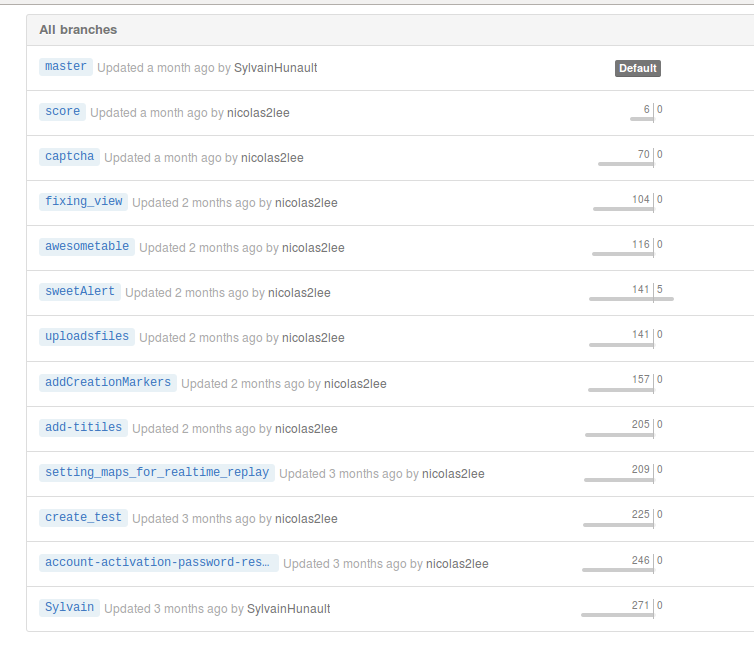
\includegraphics[width=12cm]{allbranches.png}
    \caption{All function-oriented branches }
    \label{fig-sample}
\end{figure}

%============ new features
\subsection{New features}
%============ New style and New Home Page
\subsubsection{New style and New GUI}
%\begin{figure}[h!]
%    \centering
%    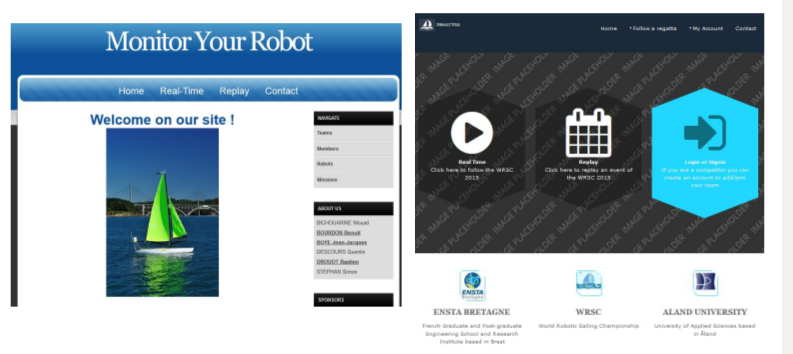
\includegraphics[width=20cm]{oldversion.png}
%    \caption{old version GUI }
%    \label{fig-sample}
%\end{figure}
\begin{figure}[h!]
\centering
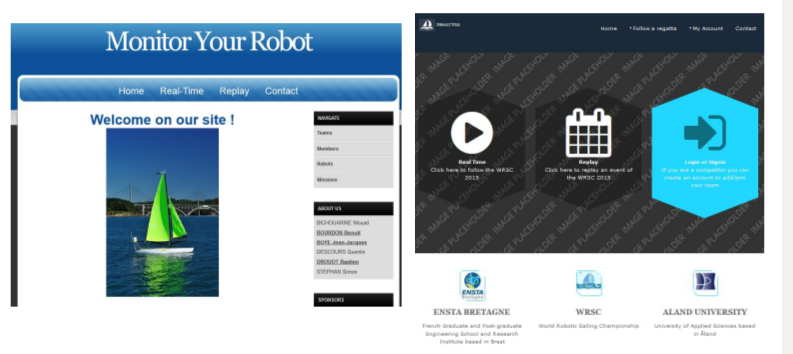
\includegraphics[width=14cm]{oldversion.png}
\caption{old home page, WRSC2014, MYR2015 }
\label{fig-sample}
\end{figure}
The web site created for the WRSC 2014 (project SWARMON) contains a no open sources CSS and Layout(left image in the figure before), and at the beginning of 2015, the web site was updated with the latest CSS3 which is open sources and more beautiful and customizable(right image in the figure before). Our current web site based on the latest CSS3.
\begin{figure}[h!]
\centering
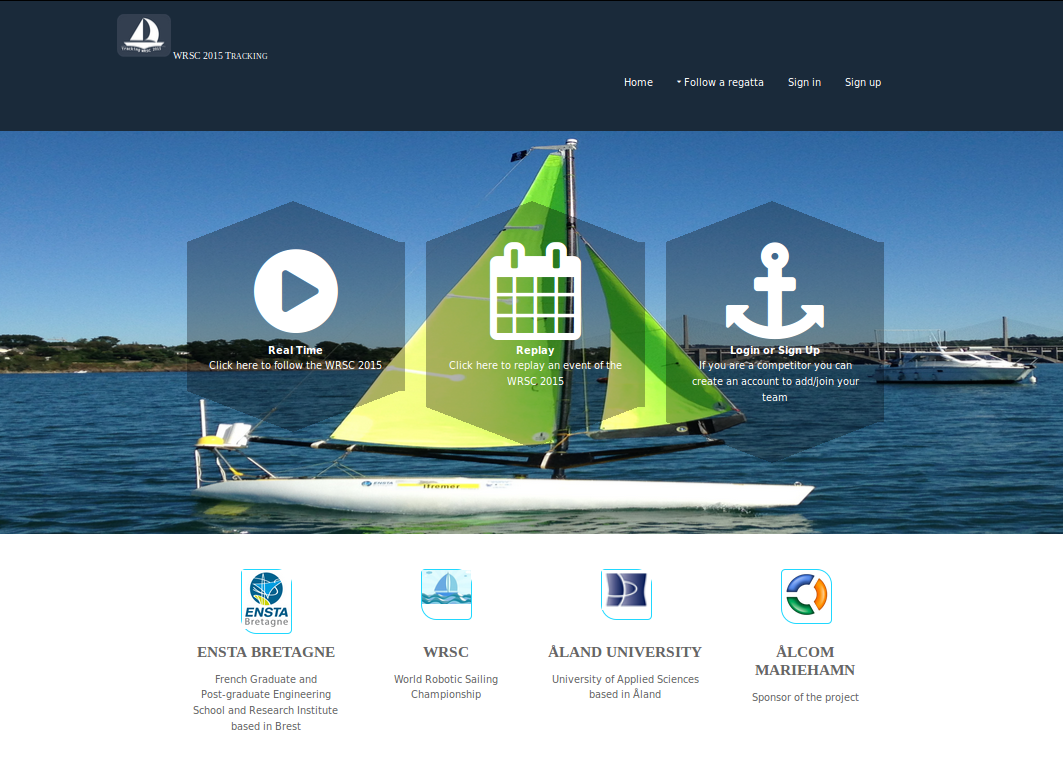
\includegraphics[width=13cm]{homepage.png}
\caption{New Home Page }
\end{figure}

%====== add team#show
\begin{figure}[h!]
\centering
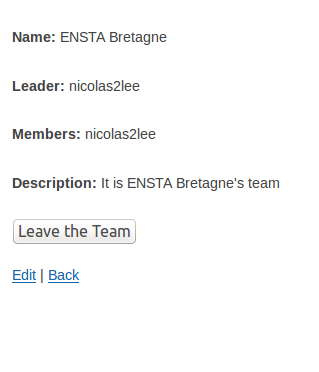
\includegraphics[width=15cm]{oldteamshow.png}
\caption{old team show}
\label{fig-sample}
\end{figure}
In the previous version, the web site could only display the basic information about every team, like: team name, leader, members and description. In order to simplify the access, we add two fields by using two Ajax requests to permit the management of members and robots, so team leader could kick their members by itself rather than ask the administrator to do so. 

%====== add robot#show
Similar to the page team\#show, the previous web site could only display the basic information about every robot, like: name, owner(team), category. These information are essential but insufficient, especially for the new visitors, the users do not know which mission their robot participated (if they want to know, they need to go to the page attempts, and check their robot name in the whole list one by one and also if they want to know the time for missions, or/and the time for every attempt, they need to go another page to check all the information). So in order to facilitate the use of web site, we decided to put all these information into the page robot\#show. Also we had thought a lot about the form to display all these information to users, since the logic is that a robot participates several missions, and for every mission, there could be more attempts, and every score and tracker id were attached to an attempt. So based on this hierarchical order, it will better to choose a tree structure chart to show the logic. In order to meet our need, we had chosen google org charts which are open sources and all APIs are provided and published by Google company. Since our web site was built up by ruby on rails, and google org charts were released as JavaScript APIs, from this, every time when the site loading the robot\#show page, it will recall a Ajax request and send all the associated information to the JavaScript part, then in the JavaScript part, we could use the org charts' APIs directly. 
\begin{figure}[h!]
\centering
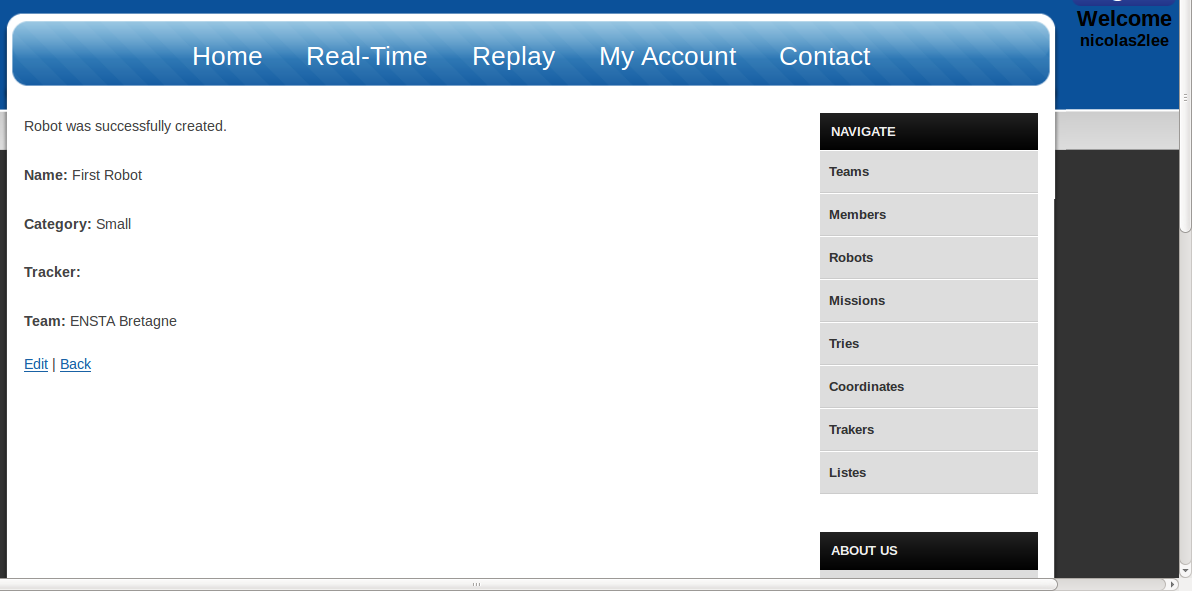
\includegraphics[width=15cm]{oldrobots.png}
\caption{old robot show}
\label{fig-sample}
\end{figure}
\begin{figure}[h!]
\centering
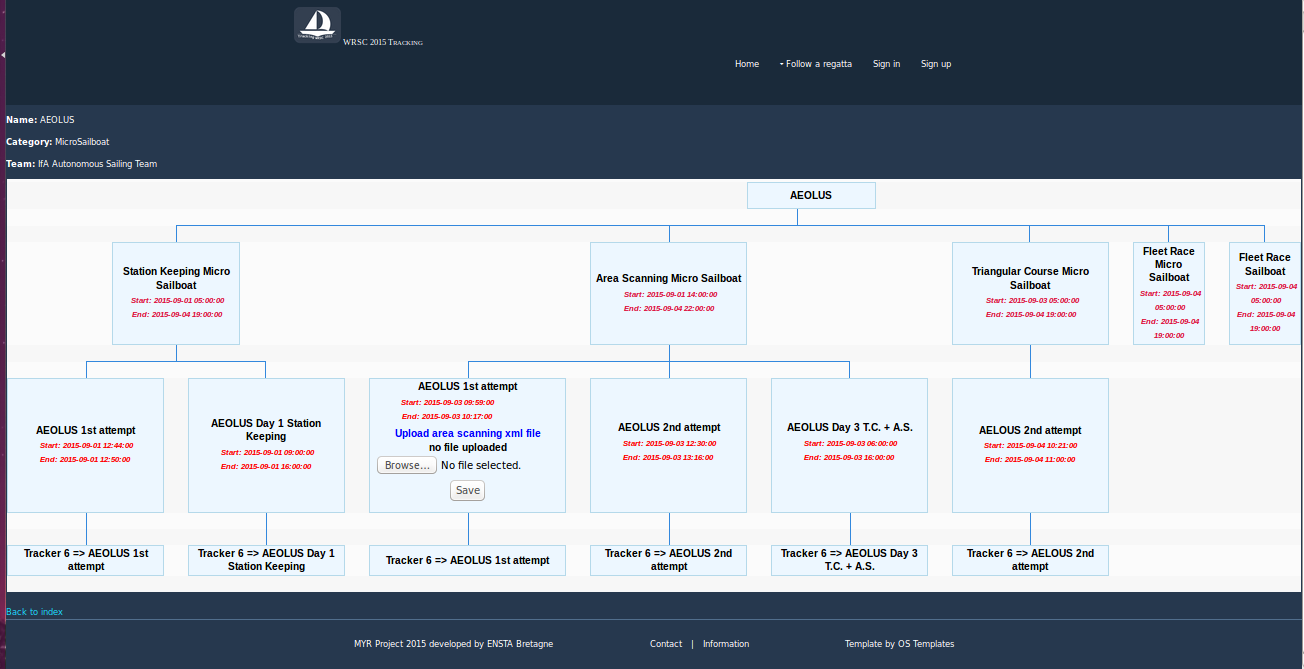
\includegraphics[width=15cm]{orgcharts.png}
\caption{Google org charts example }
\label{fig-sample}
\end{figure}

%============== Sortable \& Searchable Table
\subsubsection{Sortable \& Searchable Table}

The previous version web site(WRSC 2014 in Galway) used a table to list all the information for teams, robots, missions, members and etc. And all these tables are only sortable by the alphabetic order.
\begin{figure}[h!]
\centering
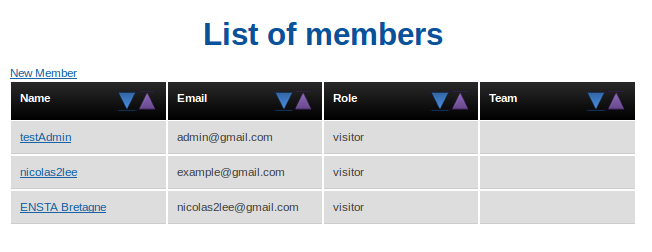
\includegraphics[width=15cm]{oldtable.png}
\caption{WRSC 2014 searchable only table }
\label{fig-sample}
\end{figure}
The only sortable table works well when there is not enormous data, if we suppose that there are more than 100 members in our database, and if you want to find the information about one member and you had only the name of this member, it will be stupid to check the whole list just by eyes. Furthermore, if the web site displays more than 10 records in one page, which often makes the user feeling uncomfortable and inefficient. Based on these reasons, we choose a flexible and customisable JavaScript plug-in "DataTable". DataTables is very simple to use as a jQuery plug-in with a huge range of customisable option, and the functions which we are interested most are sorting(which makes the table sortable by alphabetic order), filtering (which makes the table searchable, we can search one element by typing part of the keyword) and pagination (which limits the number of elements in one page, also it will make the page loading be faster and reduce the pressure of server because of the limitation of elements in the page). What's more, "DataTable" provides more APIs which also make the html table flexible, the developers are easy to get the index or element in the table just by calling the functions, comparing to the static html table, the "DataTable" is more dynamic and interacted for users.
\begin{figure}[h!]
\centering
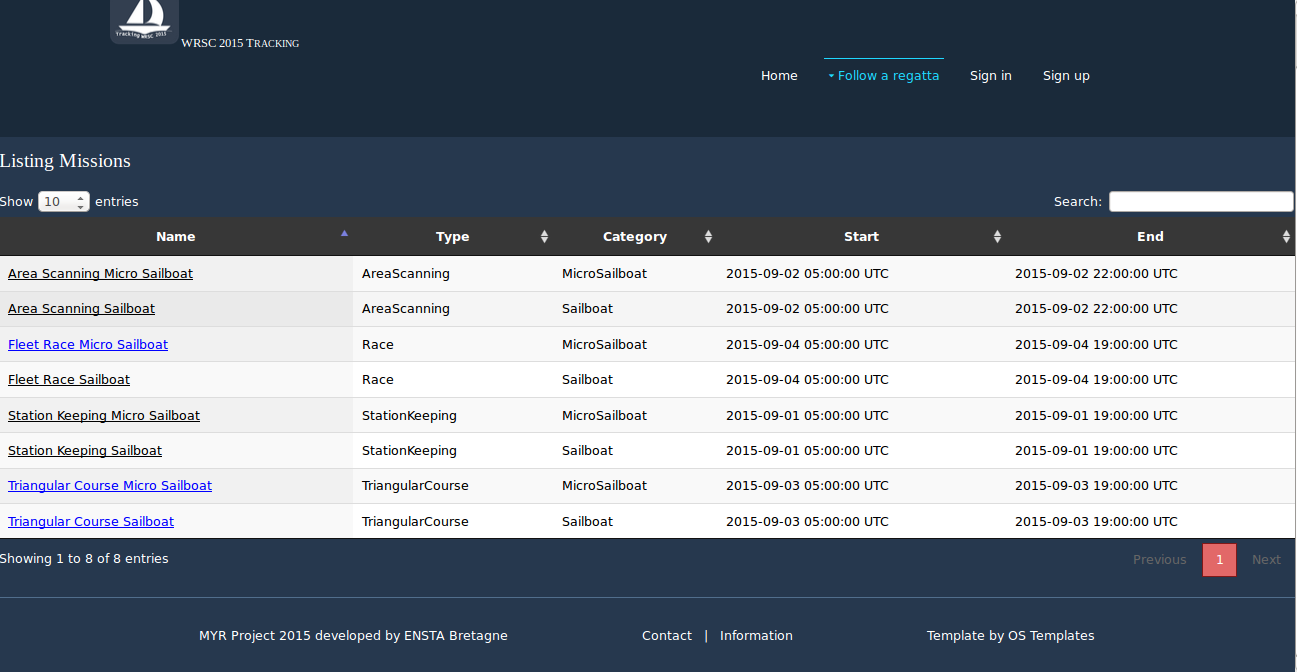
\includegraphics[width=15cm]{DataTable.png}
\caption{DataTable plug-in example }
\label{fig-sample}
\end{figure}

\subsubsection{Improved Account Management}
\begin{enumerate}
\item{Signup}
\begin{figure}[h!]
\centering
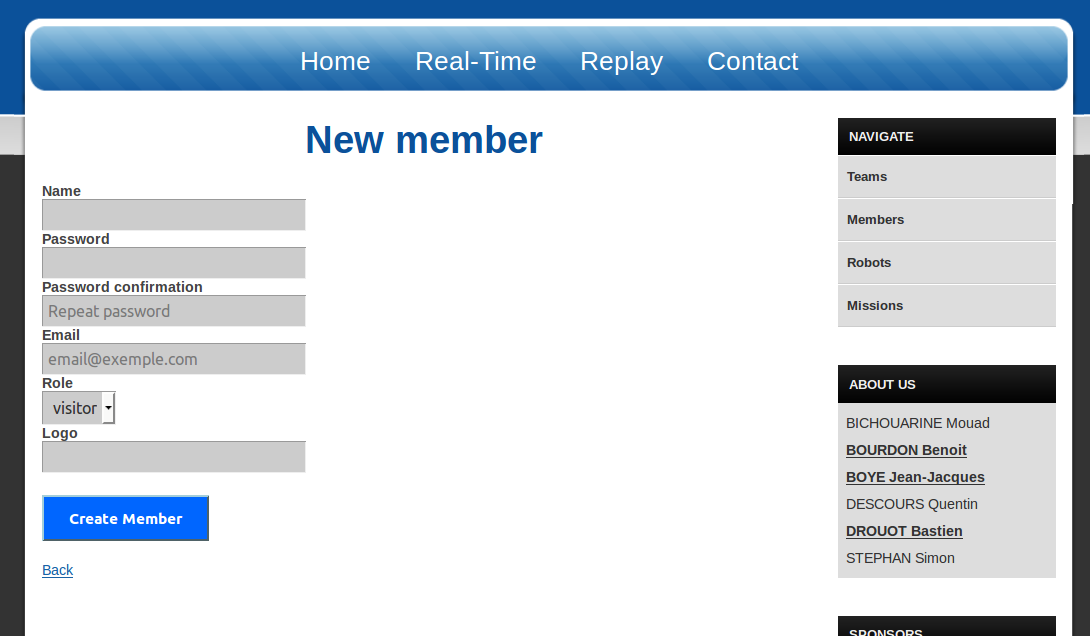
\includegraphics[width=15cm]{oldsignup.png}
\caption{old sign up }
\label{fig-sample}
\end{figure}

\begin{figure}[h!]
\centering
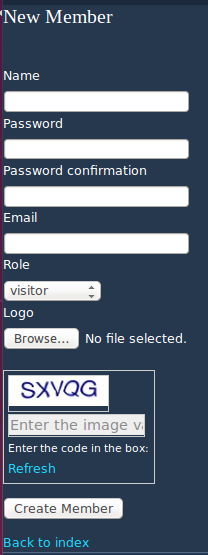
\includegraphics[width=15cm]{newsignup.png}
\caption{new sign up }
\label{fig-sample}
\end{figure}

The new sign up page add two new features:
\begin{itemize}
\item{Uploading local image file instead of typing a link}


In the old version web site, the user could only typing an image file url to upload the logo. And at the side of server, it adopts a gem called "fastimage", which could handle of the url and get the image of this url, but one limitation is the image size could not larger than several hundred pixels * several hundred pixels, as a matter of fact, this size is quite small comparing to the normal image file which is nearly several mega bytes. So for this reason, the logo field is nearly useless because of the inconvenient. 
\paragraph{Software requirements}
In the new website, we used a gem called "carrierwave"(an open sources free project, all the codes are available in their Github repertoire), which permit to upload no matter what format file. Furthermore, here we need to treat the image file, so at the side of rails application, it requires another gem "mini\_magick"(Unlike RMagick, MiniMagick is a much thinner wrapper around ImageMagick, that's why we choose MiniMagick rather than RMagick), at the side of server machine, it requires the software "ImageMagick" (under Linux, type "convert -v" to check if the "ImageMagick" was installed).
\paragraph{Apply to web site}
Once all the gems are installed successfully, a new folder "uploaders" will be added into Rails.root(the root path of rails application)/app/uploaders, and the creation of uploading action is similar to create a controller/model in rails application, either by the command "rails generate uploader nameoffile", or by create the file manually. And then in the model, we need to mount the uploader, in our case, we need to add  "mount\_uploader :logo, MemberlogoUploader" in the file Rails.root/app/models/member.rb. After that, the attribute logo of member would only accept a file uploader object, even at the beginning, we define the type of logo is a string. If we dive deep into the database(either look through by rails console, or by SQLite database browser, the attribute logo is filled by a complicated object where it contains the original file name which means the name of uploaded image file, also the name of full name which means the uploaded image file's absolute file name--path in the rails application + file name and other information). Due to this reason, once an image file was uploaded, we should not change the position of this file, because in the database, the image file was just saved as the path and the name rather than the image self.


What's more, "carrierwave" provided some other customizable convenient options, for instance, we can define our own store directory to put all the image files. Actually by default, all the files accessible for any other user should be put into Rails.root/public. But do not trust the file uploaded via internet, so we should make sure all the files in public directory were inexecutable. From this, "carrierwave" also provide an option to set the extension white list, where we can limit the file format to avoid the virus. In addition, if the rails application was launched by a Linux machine, we can set the permission of the directory public to make sure all the users except the owner(admin) could only read and write, but not execute. One way possible to do so is by using the command "chmod 766 <directory>", then with the command "ls -l", we can check if the directory permission is
"drwxrw-rw-".

Also we can define different versions of image files with different sizes based on the same image, which will be applied once the image file was uploaded.

\item{Simple captcha}
Another important change for the sign up page is that we added the captcha to filtering human user and avoid basic attacks. The realization of captcha is also simple. We used a gem called "simple\_capthca2"(an open sources free project, all the codes are also available from Github repertoire). 
As controller Based, we just need to do:
Add the following line in the file “app/controllers/application.rb”
\begin{lstlisting}
ApplicationController < ActionController::Base
  include SimpleCaptcha::ControllerHelpers
end
\end{lstlisting}

In the view file within the form tags add this code
\begin{lstlisting}
<%= show_simple_captcha %>
\end{lstlisting}

and in the controller's action authenticate it as
\begin{lstlisting}[language=Ruby]
if simple_captcha_valid?
  do this
else
  do that
end
\end{lstlisting}
\item{Activate by email}
In the new web site, also we add the function of sending emails to activate the new account when one user register on the site. As we do not have any specific email account, we choose Gmail account as our admin email account because of several reasons.
\begin{itemize}
\item In order to display the google map in our web site, we register a google account to obtain a google map JavaScript API key, so already even we did not choose Gmail as our main email, we should at least use the google account for JavaScript API.
\item Gmail service is free and easy to use, although Google limits the amount of mail a user can send, via its portable SMTP server, and the amount of sending emails is limited 99 per day, regarding our web site is focused on the participates, even maybe there are some other users, 99 is already enough for the email function. In addition, if we want much more capacity, if the budget allows, we could buy the service of Gmail SMTP server in the future.
\item Gmail is secure, wide used and compatible with others email service provider. And sometimes, Gmail is too secure to use. And the problem we meet at the beginning is that we had sent an email by configuring the SMTP server in our Rails Application, then Google detected this operation was done by machine not a web user and our email was blocked. In order to solve these types of problems, we need to configure our Gmail to less secure status by going to this page https://www.google.com/settings/security/lesssecureapps and changing to less secure.
\end{itemize}
When the Gmail account was setted correctly, and also we can send emails to other users, another problem came to our views. How can we send a unique link to the user and also how can we identify this link is associated with the relative user ? Actually before create a user, we create a new activate token(which is used to send to the user) and a activate digest(which is saved into database and used to identify the relative user). 
In the file Rails.root/app/models/member.rb
\begin{lstlisting}
	before_create :create_activation_digest
	def create_activation_digest
		self.activation_token  = Member.new_token
		self.activation_digest = Member.digest(activation_token)
	end
\end{lstlisting}
In fact, all the passwords, or more generally, the important information are encrypted before saving into the database by using the popular gem "Bcrypt". Obviously the security of encryption depends on the longer of generated token(Here we used 64 bits to generate a random token, normally it is long enough) and the algorithm(In this case, it is "Eksblowfish"--"expensive key schedule Blowfish", which based on the algorithm Blowfish. Cryptotheoretically, this is no stronger than the standard Blowfish key schedule). Also we need to pass the user's email address as an argument in the url, then we can identify the token with the member which was saved in the database found by the email address.
In the file Rails.root/app/models/member.rb
\begin{lstlisting}
    def Member.digest(string)
   		cost = ActiveModel::SecurePassword.min_cost ? 
   			   BCrypt::Engine::MIN_COST : BCrypt::Engine.cost
		BCrypt::Password.create(string, cost: cost)
    end
    
    def Member.new_token
   	 	SecureRandom.urlsafe_base64
   	end
\end{lstlisting}
Then the creation of email sending is just like any other page, firstly create the controller with desired actions, and then create the views which would be sent to the user later.
\end{itemize}

\item{Sign in}

In the new sign in page, we had also added two new features:
\begin{itemize}
\item{Remember the User}
The function of "Remember me" is quite similar to sending the activation link to users. If the user choose to remember in the computer, then the server would write the user id and a remember token into cookies, with the function cookies.signed which provided by rails application, the contents in the cookies would be encrypted. Furthermore, something should be noticed: 
\begin{itemize}
\item Cookies exist in different browsers in the same computer, so if the user has more than one browser (for instance: one Firefox and one Chrome), the cookies will be shared between the two browsers. 
\item The contents in the cookies contains two values, one is what we want to save into the cookie, and the other one is the expire date which indicates the validate time for cookie. If we use "session", which contains the same contents as cookies, but the expire date is from when the contents were created to when the user close the browser.
\end{itemize} 

\item{Reset the Password}
"Reset the password" has the similar principle as the activation email sending. When a user request to reset its password, it needs to provide its email address as a reference. Then the server generate a token and a digest, send the link which contains the user's email address and a reset token to the user. After, when the user clicked the link, the server verifies the digest with the token, if it is the correct token, then the user could change its information.
\end{itemize}
\begin{figure}[h!]
\centering
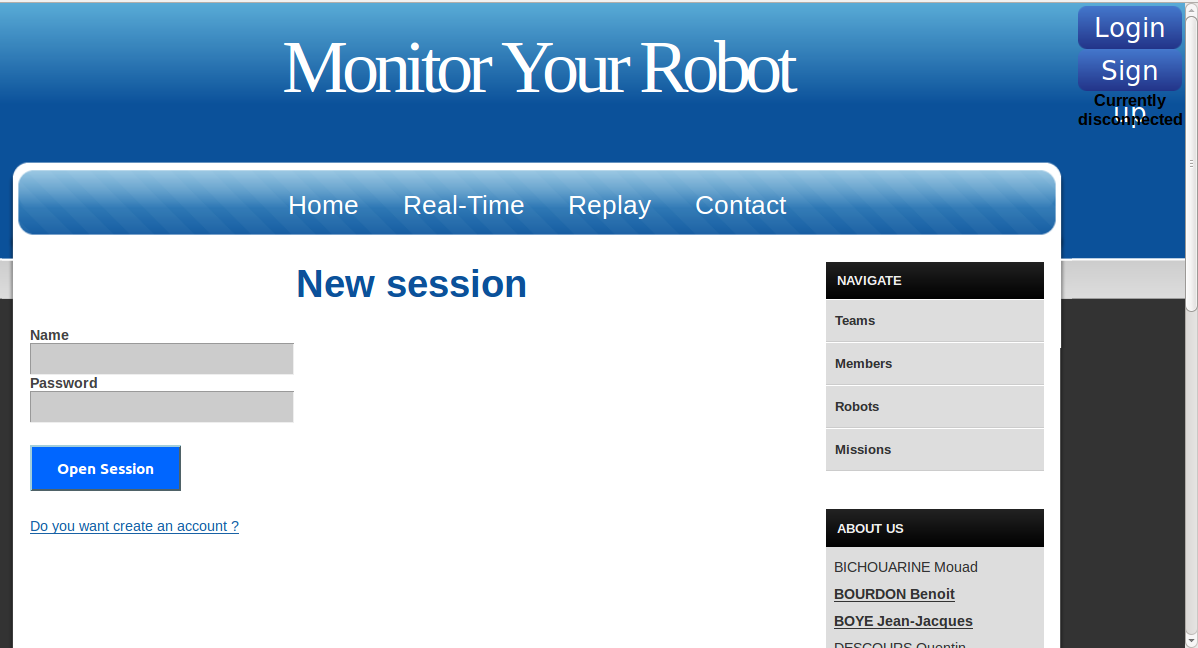
\includegraphics[width=15cm]{oldsignin.png}
\caption{old sign in }
\label{fig-sample}
\end{figure}

\begin{figure}[h!]
\centering
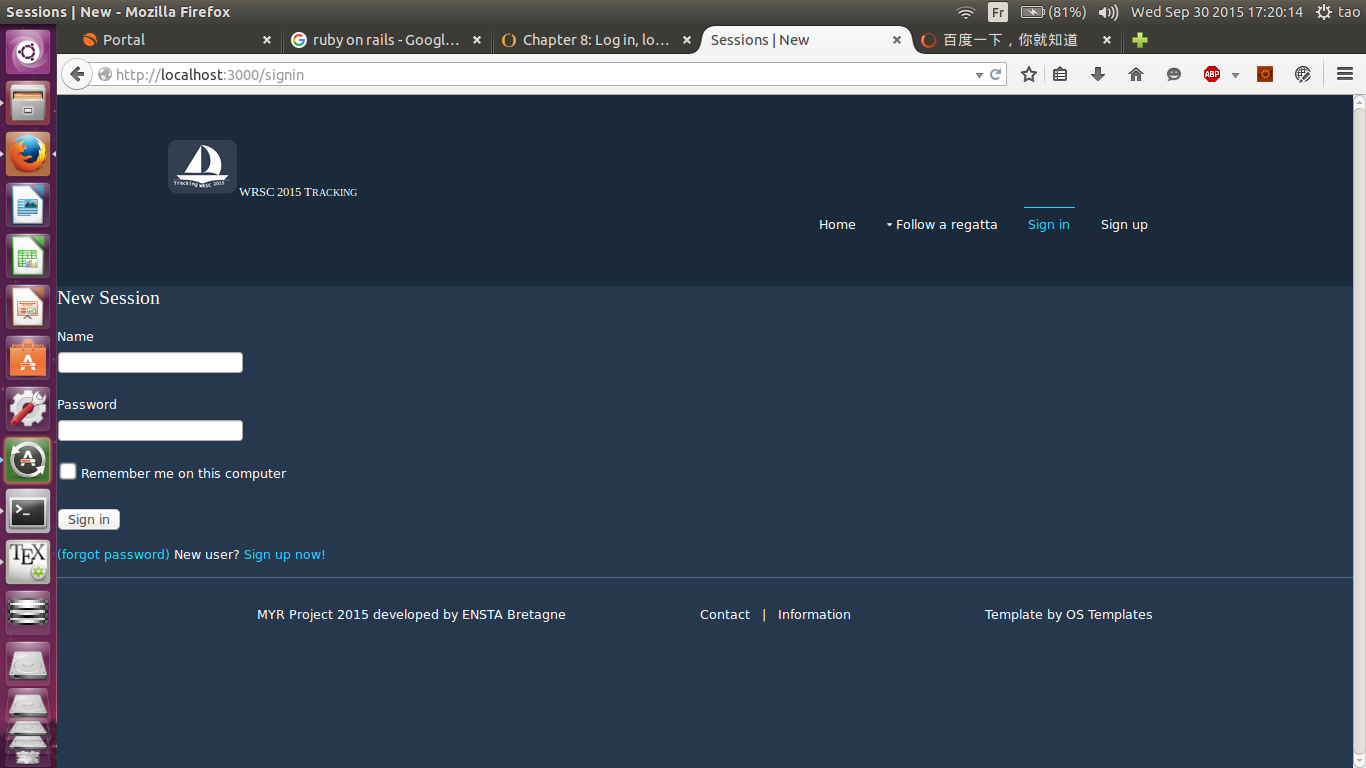
\includegraphics[width=15cm]{newsignin.png}
\caption{new sign in }
\label{fig-sample}
\end{figure}

\end{enumerate}
\subsubsection{Admin Markers Creation}
\subsubsection{Auto Scoring and Ranking}
\begin{enumerate}
\item{Scoring}


The WRSC contains 4 missions: Station Keeping, Area Scanning, Triangular Course and Fleet Race. And I was in charge of the scoring for Station Keeping and Area Scanning. So I will introduce the algorithms I had chosen to calculate the score.
\begin{itemize}
\item{Station Keeping}
\begin{itemize}
\item{Description of mission}
As the WRSC rules described, the objective of the station keeping contest is to evaluate controlled sailing in a limited region with time constraints. Each boat must start outside a 45 m x 45 m box, marked by four buoys. In the team slot time, the boat must enter the box. The boat shall leave the box at a time as close as possible to 5 minutes after entering the box. Boats fulfilling the entry and exit criteria are awarded points based on the following formula:
P = max (0, 10 - |Tenter + 300 - Tleave|/10)
Where: Tenter is the timestamp when the boat first enters the box and Tleave is the timestamp
when the boat first leaves the box. If the boat enters and leaves the box several times, any leave timestamps within ten seconds from Tenter are ignored. All timestamps are given in seconds.
\end{itemize}
\item{Area Scanning}
\begin{itemize}
\item{Description of mission}
The course will be divided into 10x10 square sections, each with a width of about 31 m. The sections will be indexed as (i, j), where i goes from 0 to 9 starting at south and going north, and j goes from 0 to 9 starting at west and going east. From the time the boat enters the first section and within a time of 90 minutes, the boat shall pass through as many square sections as possible. The score for the area scanning contest will be calculated as:
P = Npassed/10
where Npassed is the number of entered sections.
The score will be multiplied with a factor determined from oceanographic measurements provided for each visited section. Depth (m), water temperature (\textcelsius), air temperature (\textcelsius), water salinity (\%), conductivity (S/cm), chlorophyll (ug/l), ammonium (mg/l), nitrate (mg/l), chloride (mg/l) and total dissolved solids (mg/l) can be provided. Inclusion of depth data will add 0.2 to the multiplication factor, the other measurements each add 0.1. The multiplication factor is 1.0 initially, and the maximum that can be achieved is 1.5. Each team shall provide data on the team’s performance to the Race Committee within 5 hours after the start of their slot time. The data shall be in XML, specified by the schema below. The data will contain the team name. For each entered square section the section’s indices are required along with a UTC timestamp and corresponding coordinates using <gml:pos> property in WGS-84 (EPSG:4326). Optionally the oceanographic data can be added. Each entered section shall be added only once to the XML data.
\item{algorithm for Area Scanning}
Actually, for the contest area scanning, the Race Committee decided to do the scoring by themselves, but they ask us to verify the GPS data submitted by the teams with XML format with data gathered by our trackers. Fortunately, Åland University of Applied Sciences(ÅUAS) had a python program which can analyse the submitted XML file and then generate a JSON file(which contains all the useful data and this file is easy to be handled by ruby on rails). And then I based on this JSON file, compare the data with the correspondent tracker's data to check if the gaps of positions were under the tolerance. In order to accomplish this task, several steps were adopted:
\begin{enumerate}
\item The participated team should uploading their XML file to their robot's page

(robot\#IdOfTheirRobot). And also I added a time stamp to record the time when the team submitted their XML file because the team should upload their XML file in 5 hours since they had finished their attempts.
\item With python program(provided by Conny Ljunggren, ÅUAS), I need to generate a JSON file manually. Also I had looked into the python program, in fact the python program used a module called "xml.etree.ElementTree", the key point of this program is using this module to analyse XML file. Unfortunately, I did not find any similar module in Ruby to analyse the XML file, but it was also feasible in ruby. It was just like a compilation project, the code source is XML file, and then the target file is JSON file, so then if we define the grammar of XML, define the lexer and Backus Normal Form(BNF), from the Backus Normal Form(BNF), create the parser to analyse the code source, and store all the separate data in the node of Abstract Syntax Tree(AST), then either by using the visitor pattern, or mix erb with visitor pattern, we can generate the target code finally. Since we did not have so much more time, I did not realize this function.
\item Based on the JSON file, ruby could import the JSON file directly, then I can compare the GPS data to the data in our web site and calculate the difference between the two sets of data. Because all the unities of GPS data are in degree, which are incomprehensible for humans, then I transfer the unity in degree to the unity in meter by using the algorithm proposed by this site: 
http://www.movable-type.co.uk/scripts/latlong.html

\begin{figure}[h!]
    \centering
    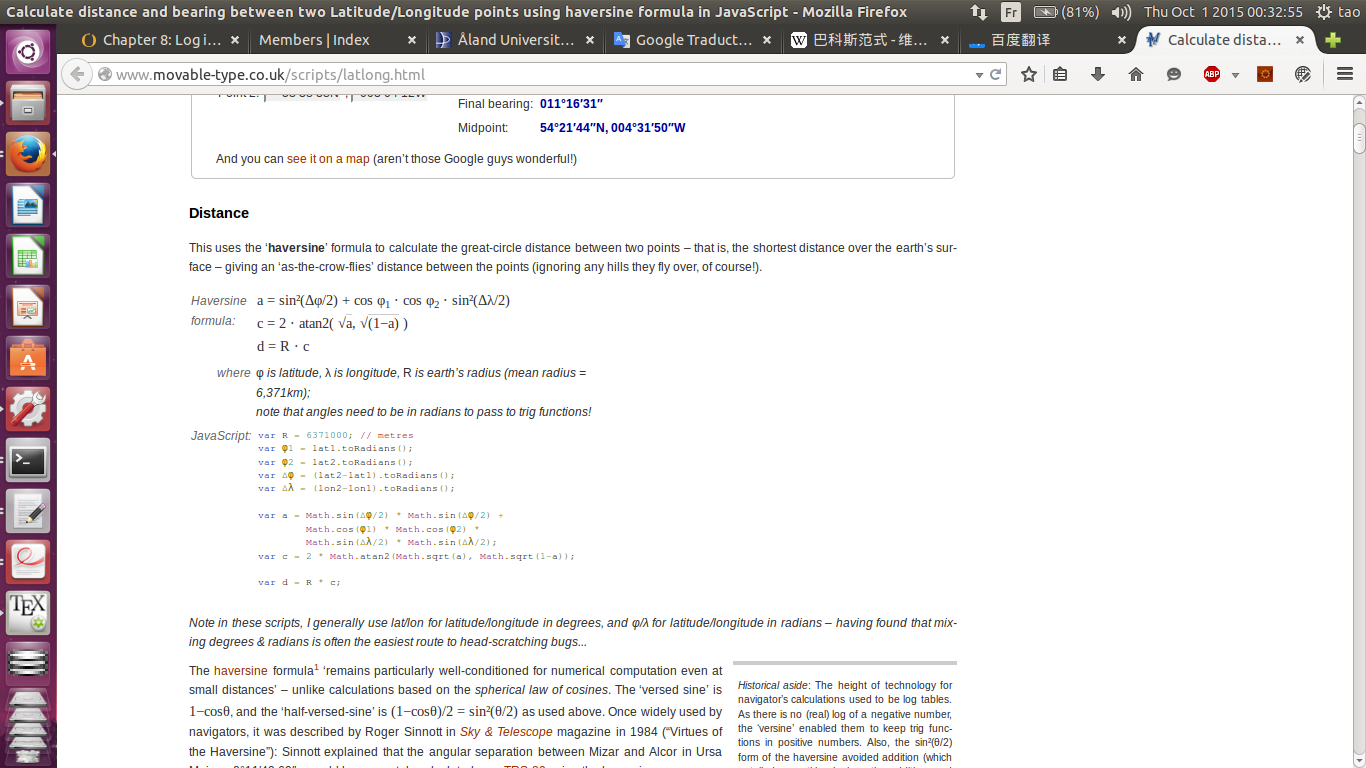
\includegraphics[width=12cm]{distanceformula.png}
    \caption{latitude longitude to meter formula from Internet}
    \label{fig-sample}
\end{figure}
And also I had tried the official contest's buoys positions. In fact, the Race Committee declared officially the distance between two buoys is about 31m [(60.1050,19.9500);(60.1080,19.9500)], and from the formula, I obtain the distance is a little more than 30m, so the gap is less than 1m which is acceptable by the GPS precision.
\item After the comparison, in ruby there are three possibilities(JSON/YAML/XML) to display the result, finally I choose XML not only to keep coherent with what they submitted, but also easy to read for users. As a matter of fact, files are also like any other resource in the web site(like views), according to the path in the rails application, we can visit the file by typing the url Rails.root/FilePath.
\end{enumerate}
 
\end{itemize}
\end{itemize} 
\end{enumerate}



%============= Une description de l'activite et des resultats du stage
\section{Reflection}
\subsection{Perspective}
Although our web site was improved greatly, but the amelioration is always existing.
\begin{enumerate}
\item{Security}
The security is always the most important thing to do. Several actions could be adopted.
\begin{itemize}
\item{HTTPS Protocol}
Foe the users' sign in and sign up pages, they should be applied the HTTPS protocol to provide a white list to avoid attackers.
\item{Robots Exclusion Protocol}
Robots exclusion protocol is used to define what we want to be quoted by the search engine (like google, yahoo). Some admin parts of the web site and also some private data do not hope to be published into the internet, then we can define the contents what we hope not to be visited by the search engine in robot.txt, and put this file into the Rails.root path. 
\begin{figure}[h!]
    \centering
    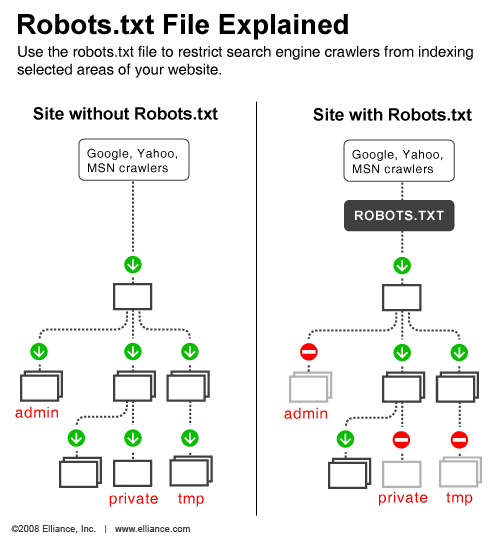
\includegraphics[width=12cm]{robot.jpg}
    \caption{All function-oriented branches }
    \label{fig-sample}
\end{figure} 
\end{itemize} 
\end{enumerate}
\subsection{Industrial analyse}
After WRSC, occasionally discussed with some Finnish engineers, we found out that they had developed a similar tracking product in order to follow the trace(http://www.thingsee.com/). Comparing our tracking system with their product, they are nearly the same, except their product contains more sensors, so they can measure more parameters, like: temperature, motion and so on, and the price of product is more than 300 Euros. Although our tracking system do not have so much sensors, but it cost much less than their product, the price of our tracking system is less than 100 Euros.
Furthermore, we found another similar project from the internet, in Brittany, France.(https://www.gwenneg.bzh/fr/tifiz) So it was not impossible to develop our own product in the near future.
\subsection{Personal analyse}
I am glad to have such a good opportunity to take part in a passionate project and also I am glad to be in Aland, Finland for my internship where I discovered a beautiful place with friendly awesome people. This impressive experience not only reinforces what I had learned, but also permit me to discover the world, to learn how real engineers realize their aims and especially work professionally under pressures.
%============= Une analyse économique de l'entreprise
%============= Une analyse de l'apport du stage pour le projet professionnel de l'etudient
\section{Conclusion}
Based on a ruby on rails framework, with jQuery libraries, building up a web server is not simple as what we see. In order to make a good product, we need to familiar with font end design technologies(html, CSS, JavaScript). Especially all the new technologies are born quickly, vast solutions and enormous tools appear. Even sometimes, it will be a little hard to struggle with the latest techniques and run after time, but keep a positive attitude to face the new things and get the capacity to filter the important information in such a big data era would be the key to success. In addition, script programming, knowledge of database and network, all of them are the basic elements to construct the final building. A wide view of multi-domains will facilitate the innovation.

Personally I am quite satisfied with what I had done. Every one or two weeks, a new feature was added, in other words, I got many different experience every one or two weeks. But also I discover the importance of test and management of project. The quality is much more important than the quantity. A few stable functions will be much better than a lot features which could not work. Further, the tests play a really important role in the development, before this internship, I thought the test time could not more than the development, it could only reach half of the whole period, but in the reality, the developers always pass most of time to check. What's more, it is impressive to work with kind and smart people in such a beautiful country. 

A full stack engineer is not only an expert in a domain, but also should be familiar with different fields, then be capable to adapt to different environment and be capable to work under pressure. This internship not only allow me to learn much more scientific technologies, but also a good experience to be a responsible engineer.

%============= Conclusion
%============= annexe
\newpage
\section{Reference}

[1] Benoit B, Quentin D, Simon S, Mouad B and Jean-Jacques B, "Projet SWARMON - Rapport de Projet", 6 June 2014
 \medskip
 
[2] Benoit B, Bastien D, "Final Report SWARMFRAME Project", 2015
 \medskip

[3] Michael Hartl, "Ruby on Rails Tutorial: Learn Web Development with Rails", 3rd version, 2014 - \url{https://www.railstutorial.org/book}
 \medskip

[4] Darel Rex Finley,"Point-In-Polygon Algorithm — Determining Whether A Point Is Inside A Complex Polygon", 2007 - \url{http://alienryderflex.com/polygon/}
 \medskip

[5] "Calculate distance, bearing and more between Latitude/Longitude points", visit on Aug 20, 2015 - \url{http://www.movable-type.co.uk/scripts/latlong.html}
 \medskip

[6] "Rules for World Robotic Sailing Championship 2015", May 09, 2015 - \url{http://wrsc2015.com/wp-content/uploads/2015/02/RulesWRSC2015May9.pdf}

\newpage
\section{Appendices}
\begin{itemize}

\item{\textbf{Appendix 1}}

All the referred projects and the projects mentioned in the article

\item{\textbf{Appendix 2}}

Versions about Ruby on Rails

\item{\textbf{Appendix 3}}

The Python Program used to generate JSON file with an input XML file

\item{\textbf{Appendix 4}}

Internship Agreement

\item{\textbf{Appendix 5}}

Assessment Report

\end{itemize}
\newpage
\subsection{All the referred projects and the projects mentioned in the article}
\begin{enumerate}
\item{\textbf{JQuery}}

A fast, small, and feature-rich JavaScript library(\url{https://jquery.com/})

\item{\textbf{Google Map JavaScript APIs}}

Provided by Google freely, enormous APIs associated with google map(\url{https://developers.google.com/maps/documentation/javascript/tutorial}) 

\item{\textbf{Google chart}}

Provided by Google freely, enormous APIs for many different types of graphs(\url{https://developers.google.com/chart/interactive/docs/})

\item{\textbf{SWARMON}}

A second year students' project realised by Benoit BOURDON, Quentin DESCOURS, Simon STEPHAN, Mouad BICHOUARINE and Jean-Jacques BOYE, under the supervision of Olivier REYNET at ENSTA Bretagne, aims to provide a tracking system for WRSC

\item{\textbf{MYR}}

A 3rd year students' project at ENSTA Bretagne based on the SWARMON by Bastien DROUOT and Benoit BOURDON, which aims to enhance the development of web site of tracking system and create a web generator for monitoring robot(\url{https://github.com/Sylyon/MYR})

\item{\textbf{DataTable}}

A project based on the jQuery JavaScript libraries aims to create a dynamic and interacted data table with any html table(\url{http://datatables.net/})

\item{\textbf{Carrierwave}}

A gem(open source and free to use) for ruby on rails makes easier to control the uploading files to the sites based on rails framework(\url{https://github.com/carrierwaveuploader/carrierwave})

\item{\textbf{Mini\_magick}}

A light gem(open source and free to use)  and a ruby wrapper for ImageMagick or GraphicsMagick(\url{https://github.com/minimagick/minimagick})

\item{\textbf{Simple\_captcha}}

A gem(open source and free to use)  easy to add captcha into web sites based on rails framework(\url{https://github.com/galetahub/simple-captcha})

\item{\textbf{Noun}}

A project offers enormous awesome icons(\url{https://thenounproject.com/})

\item{\textbf{Favicon}}

A project offers awesome icons which could be inserted easily into html code(\url{http://fortawesome.github.io/Font-Awesome/3.2.1/examples/})

\item{\textbf{Current Web site}}

All the codes are in my Github repertoire(\url{https://github.com/nicolas2lee/AdvancedMYR}) 
\end{enumerate}
\subsection{Versions about Ruby on Rails}
Actually my work environment is ubuntu 14.04.
In order to install ruby on rails, I used rvm which is easy to control the version of ruby.
All the versions about ruby on rails for WRSC 2015 are listed below:

\begin{lstlisting}
rvm -v:

rvm 1.26.11 (latest) by Wayne E. Seguin <wayneeseguin@gmail.com>, Michal Papis <mpapis@gmail.com> [https://rvm.io/]


ruby -v:

ruby 2.1.1p76 (2014-02-24 revision 45161) [i686-linux]


rails -v:

Rails 4.2.3
\end{lstlisting}
\newpage
\subsection{The Python Program used to generate JSON file with an input XML file}
This program is which I used to generate a JSON file from a XML file during WRSC.
\begin{lstlisting}
#Author is Conny Ljunggren, Aland University of Applied Sciences - Finland
namespaces = {'gml': 'http://www.opengis.net/gml'}
import json
import xml.etree.ElementTree as ET

tree = ET.parse('XML_IfA_Sailing_2stAttempt.xml')
root = tree.getroot()

data = []
for section in root.findall('Section'):
	si = section.find('sectioni').text
	sj = section.find('sectionj').text
	timeString = section.find('dateTime').text
	timeCleaned = timeString.replace('-', '').replace('T', '').replace(':', '').replace('Z', '')
	
	position = section.find('gml:pos', namespaces).text
	latitude = float(position.split()[0])
	longitude = float(position.split()[1])
	data.append({"sectioni":si, "sectionj":sj, "position":[{"latitude":latitude, "longitude":longitude, "datetime":timeCleaned}]})

fullData = {"tracker_id":"6", "name":"IfA_Sailing", "data":data}

with open('XML_IfA_Sailing_2ndAttempt.json', 'w') as outfile:
    json.dump(fullData, outfile)
\end{lstlisting}
\subsection{Internship Agreement}
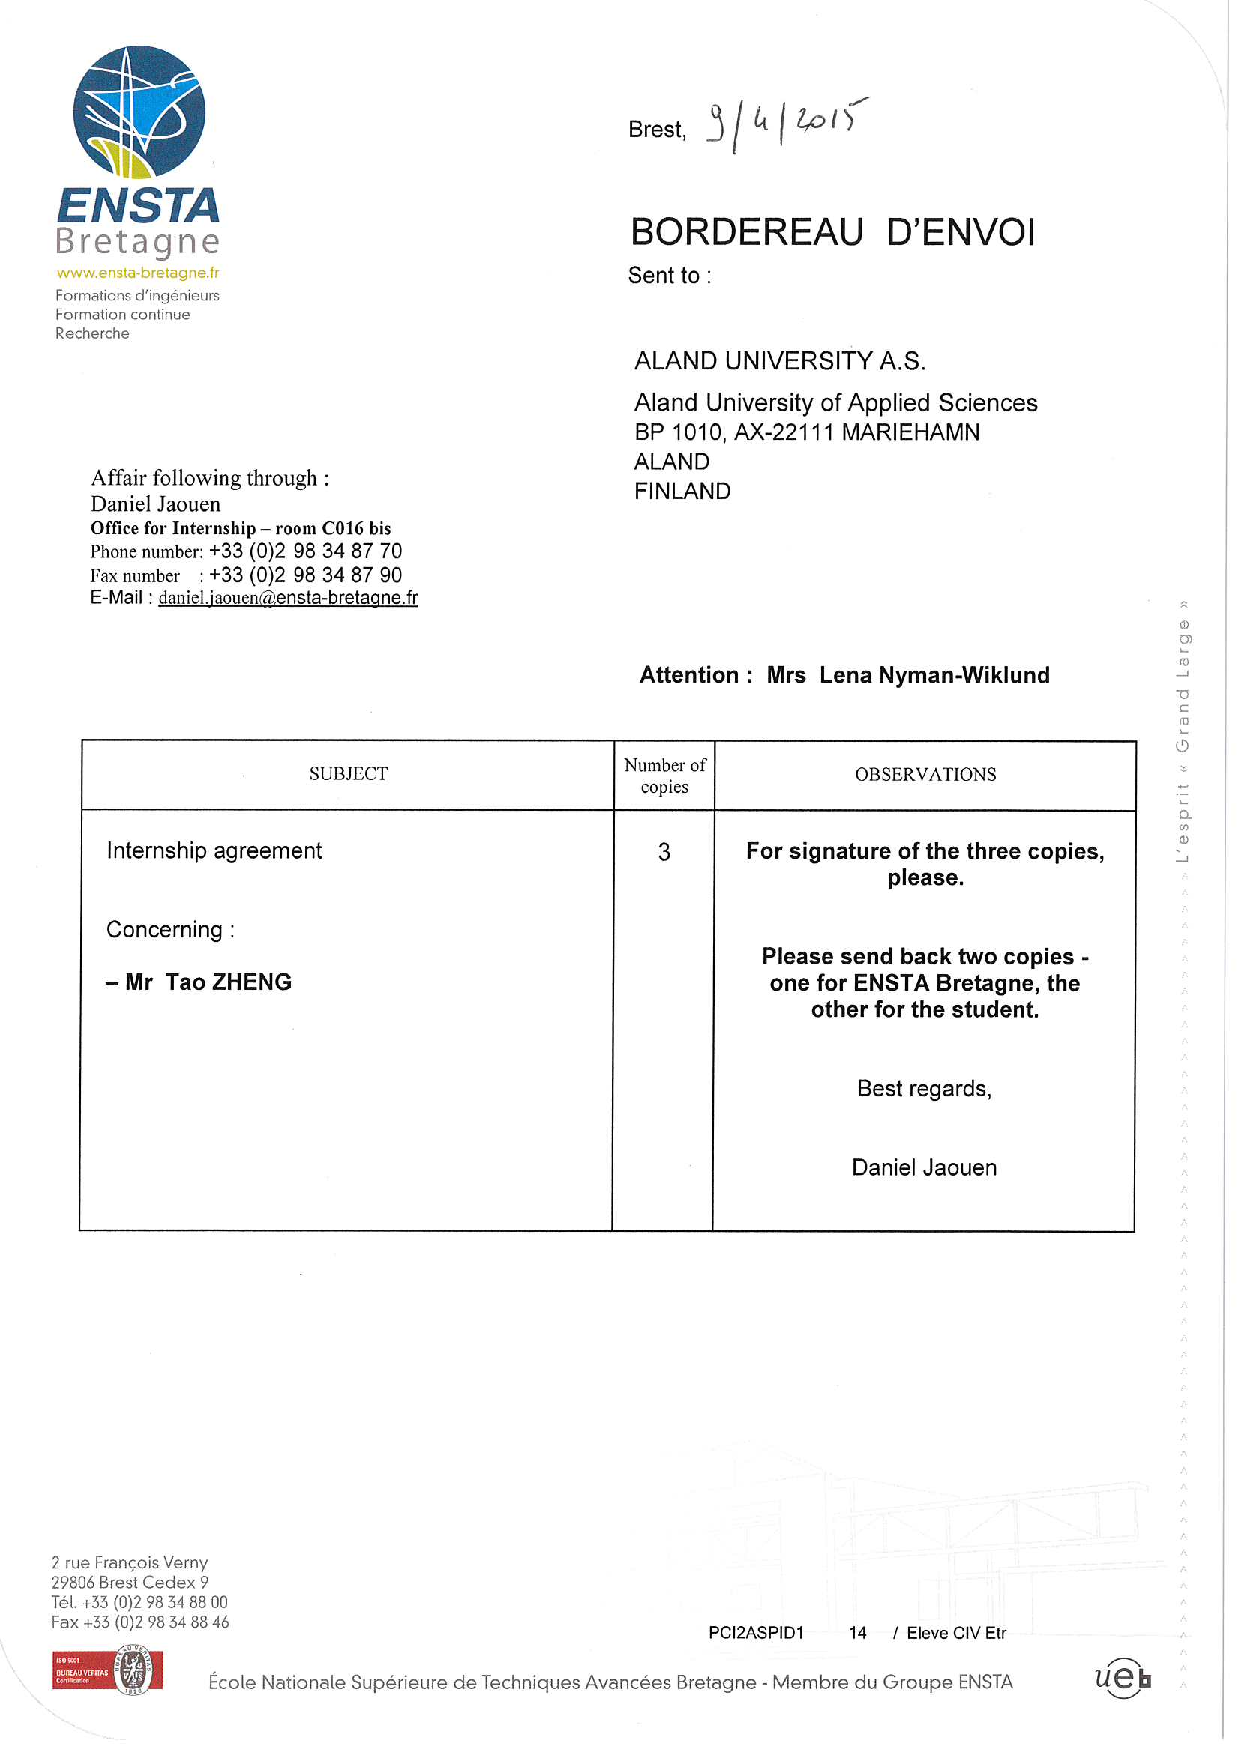
\includepdf[page=3-9]{internshipagreement.pdf}


\subsection{Assessment Report}
\begin{figure}[h!]
    \centering
    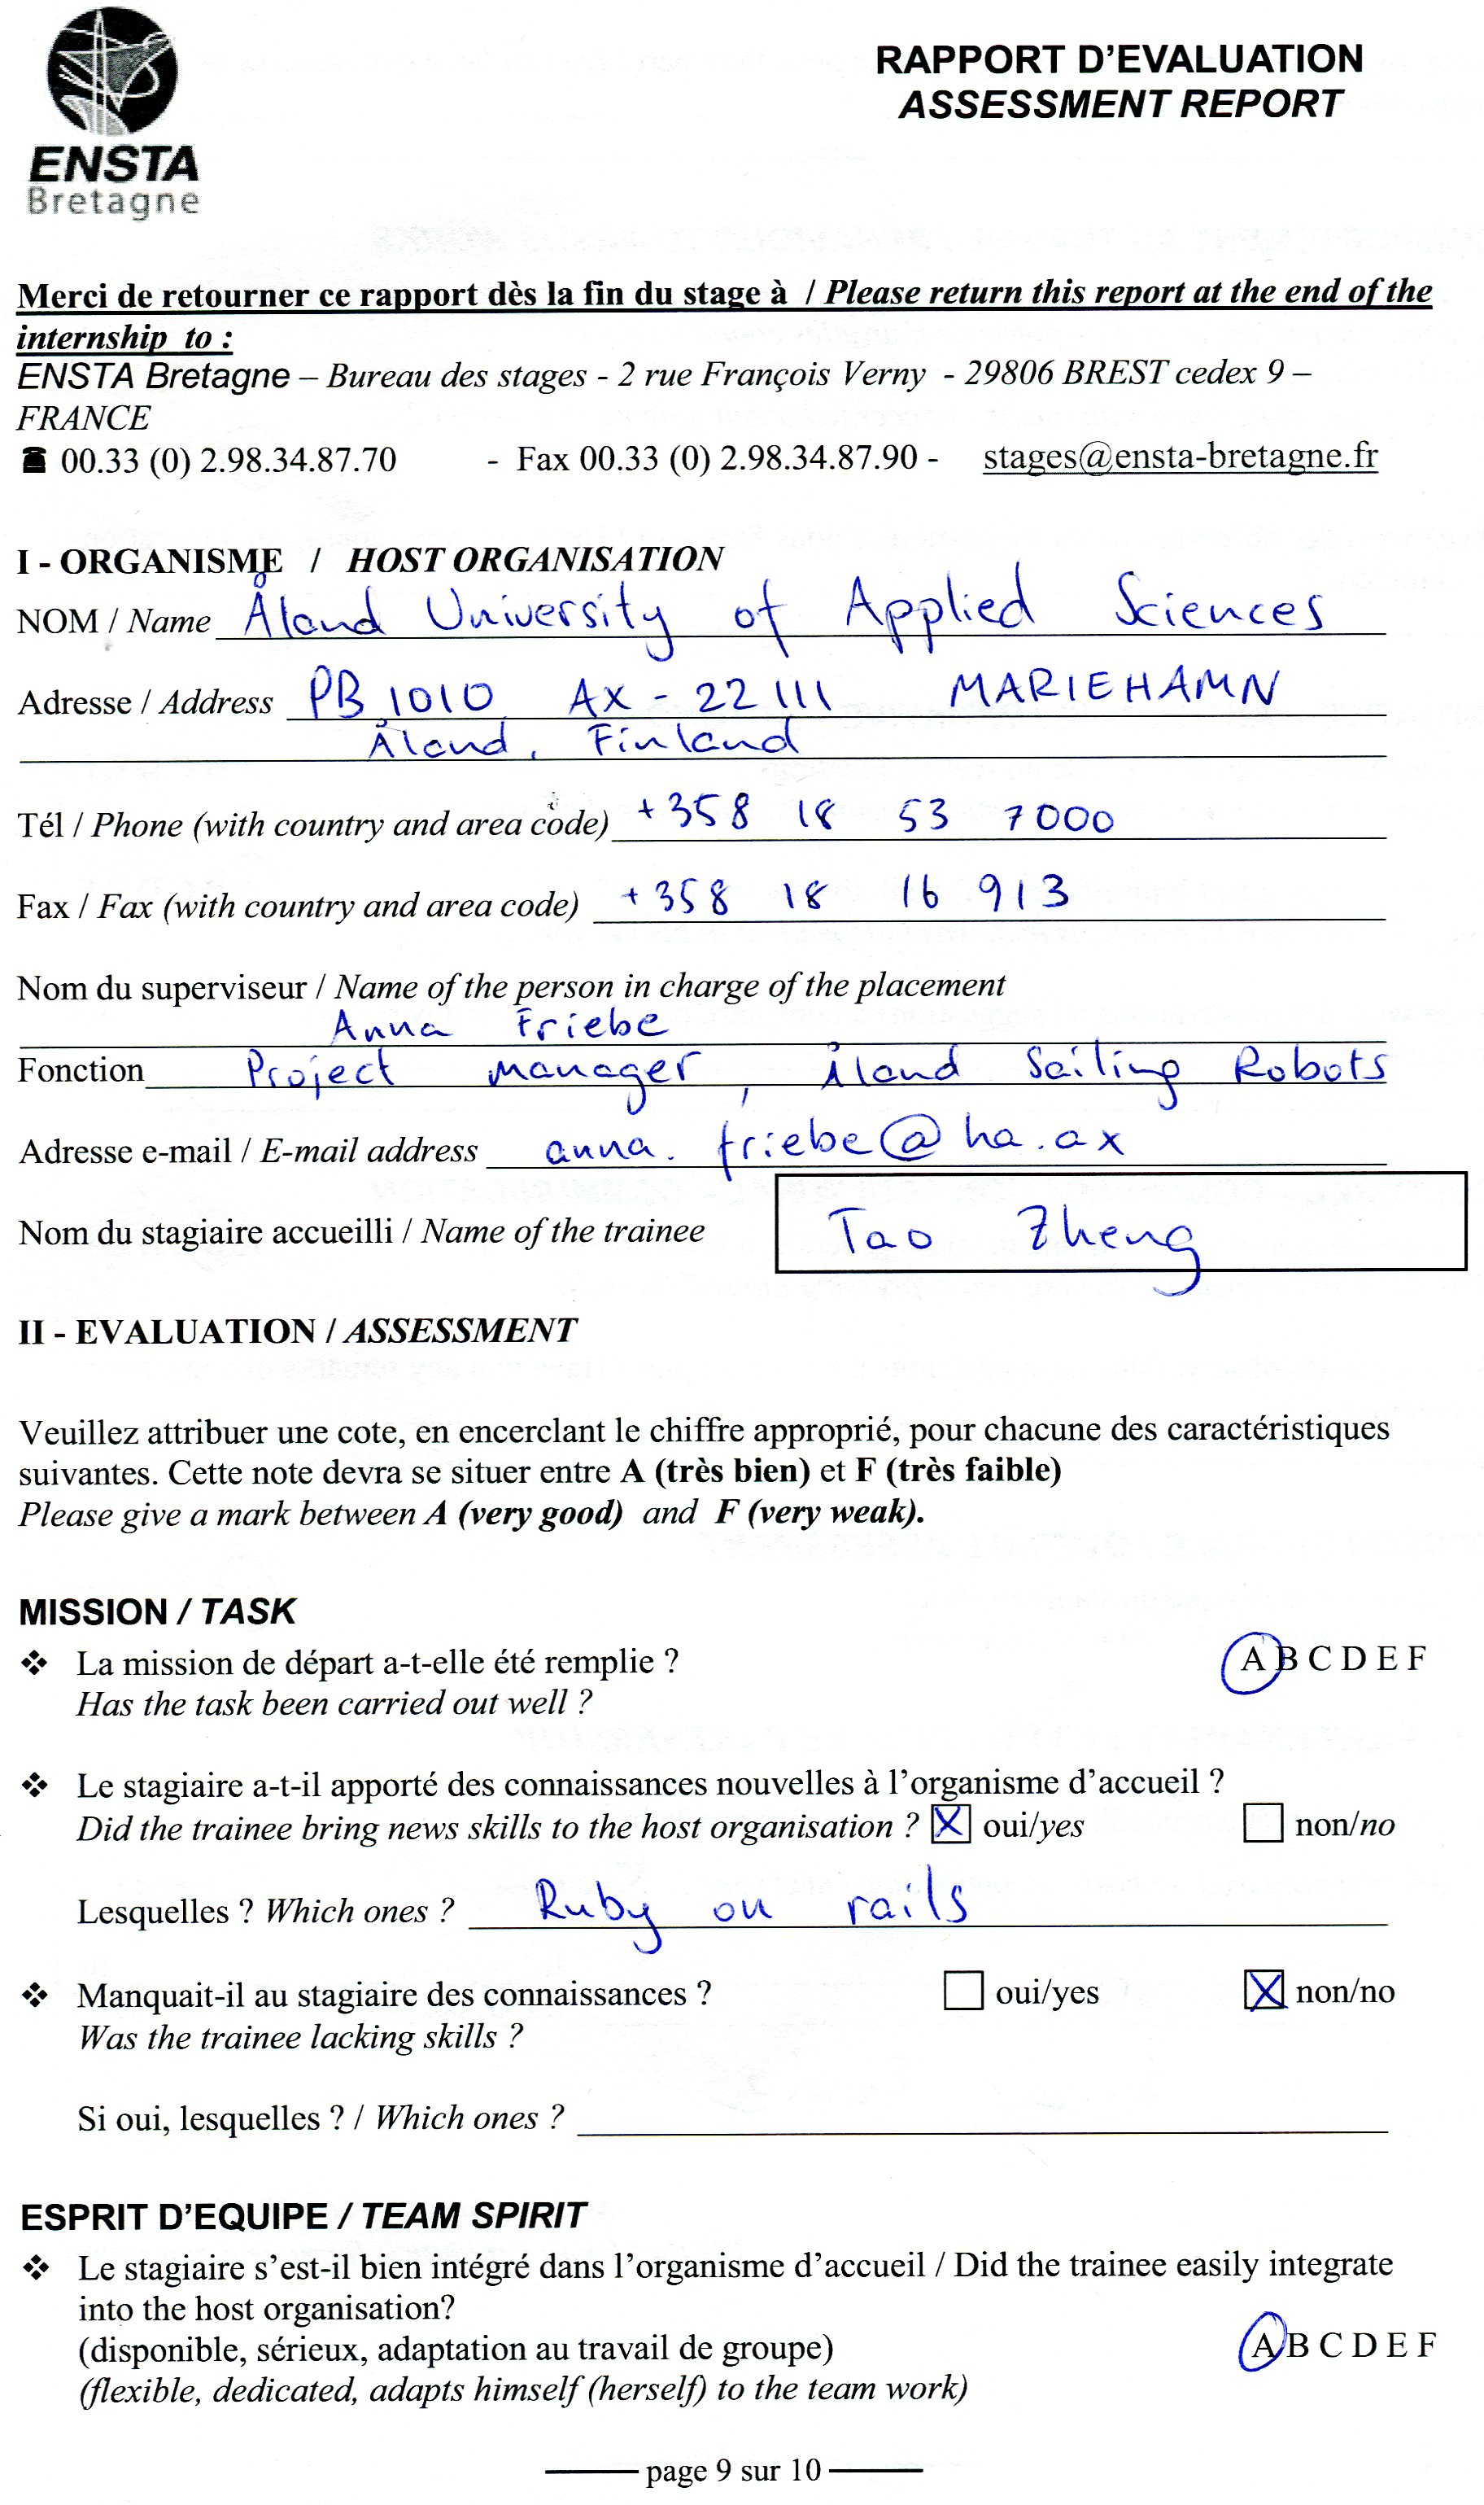
\includegraphics[width=12cm]{verso.jpg}
    \label{fig-sample}
\end{figure}
\begin{figure}[h!]
    \centering
    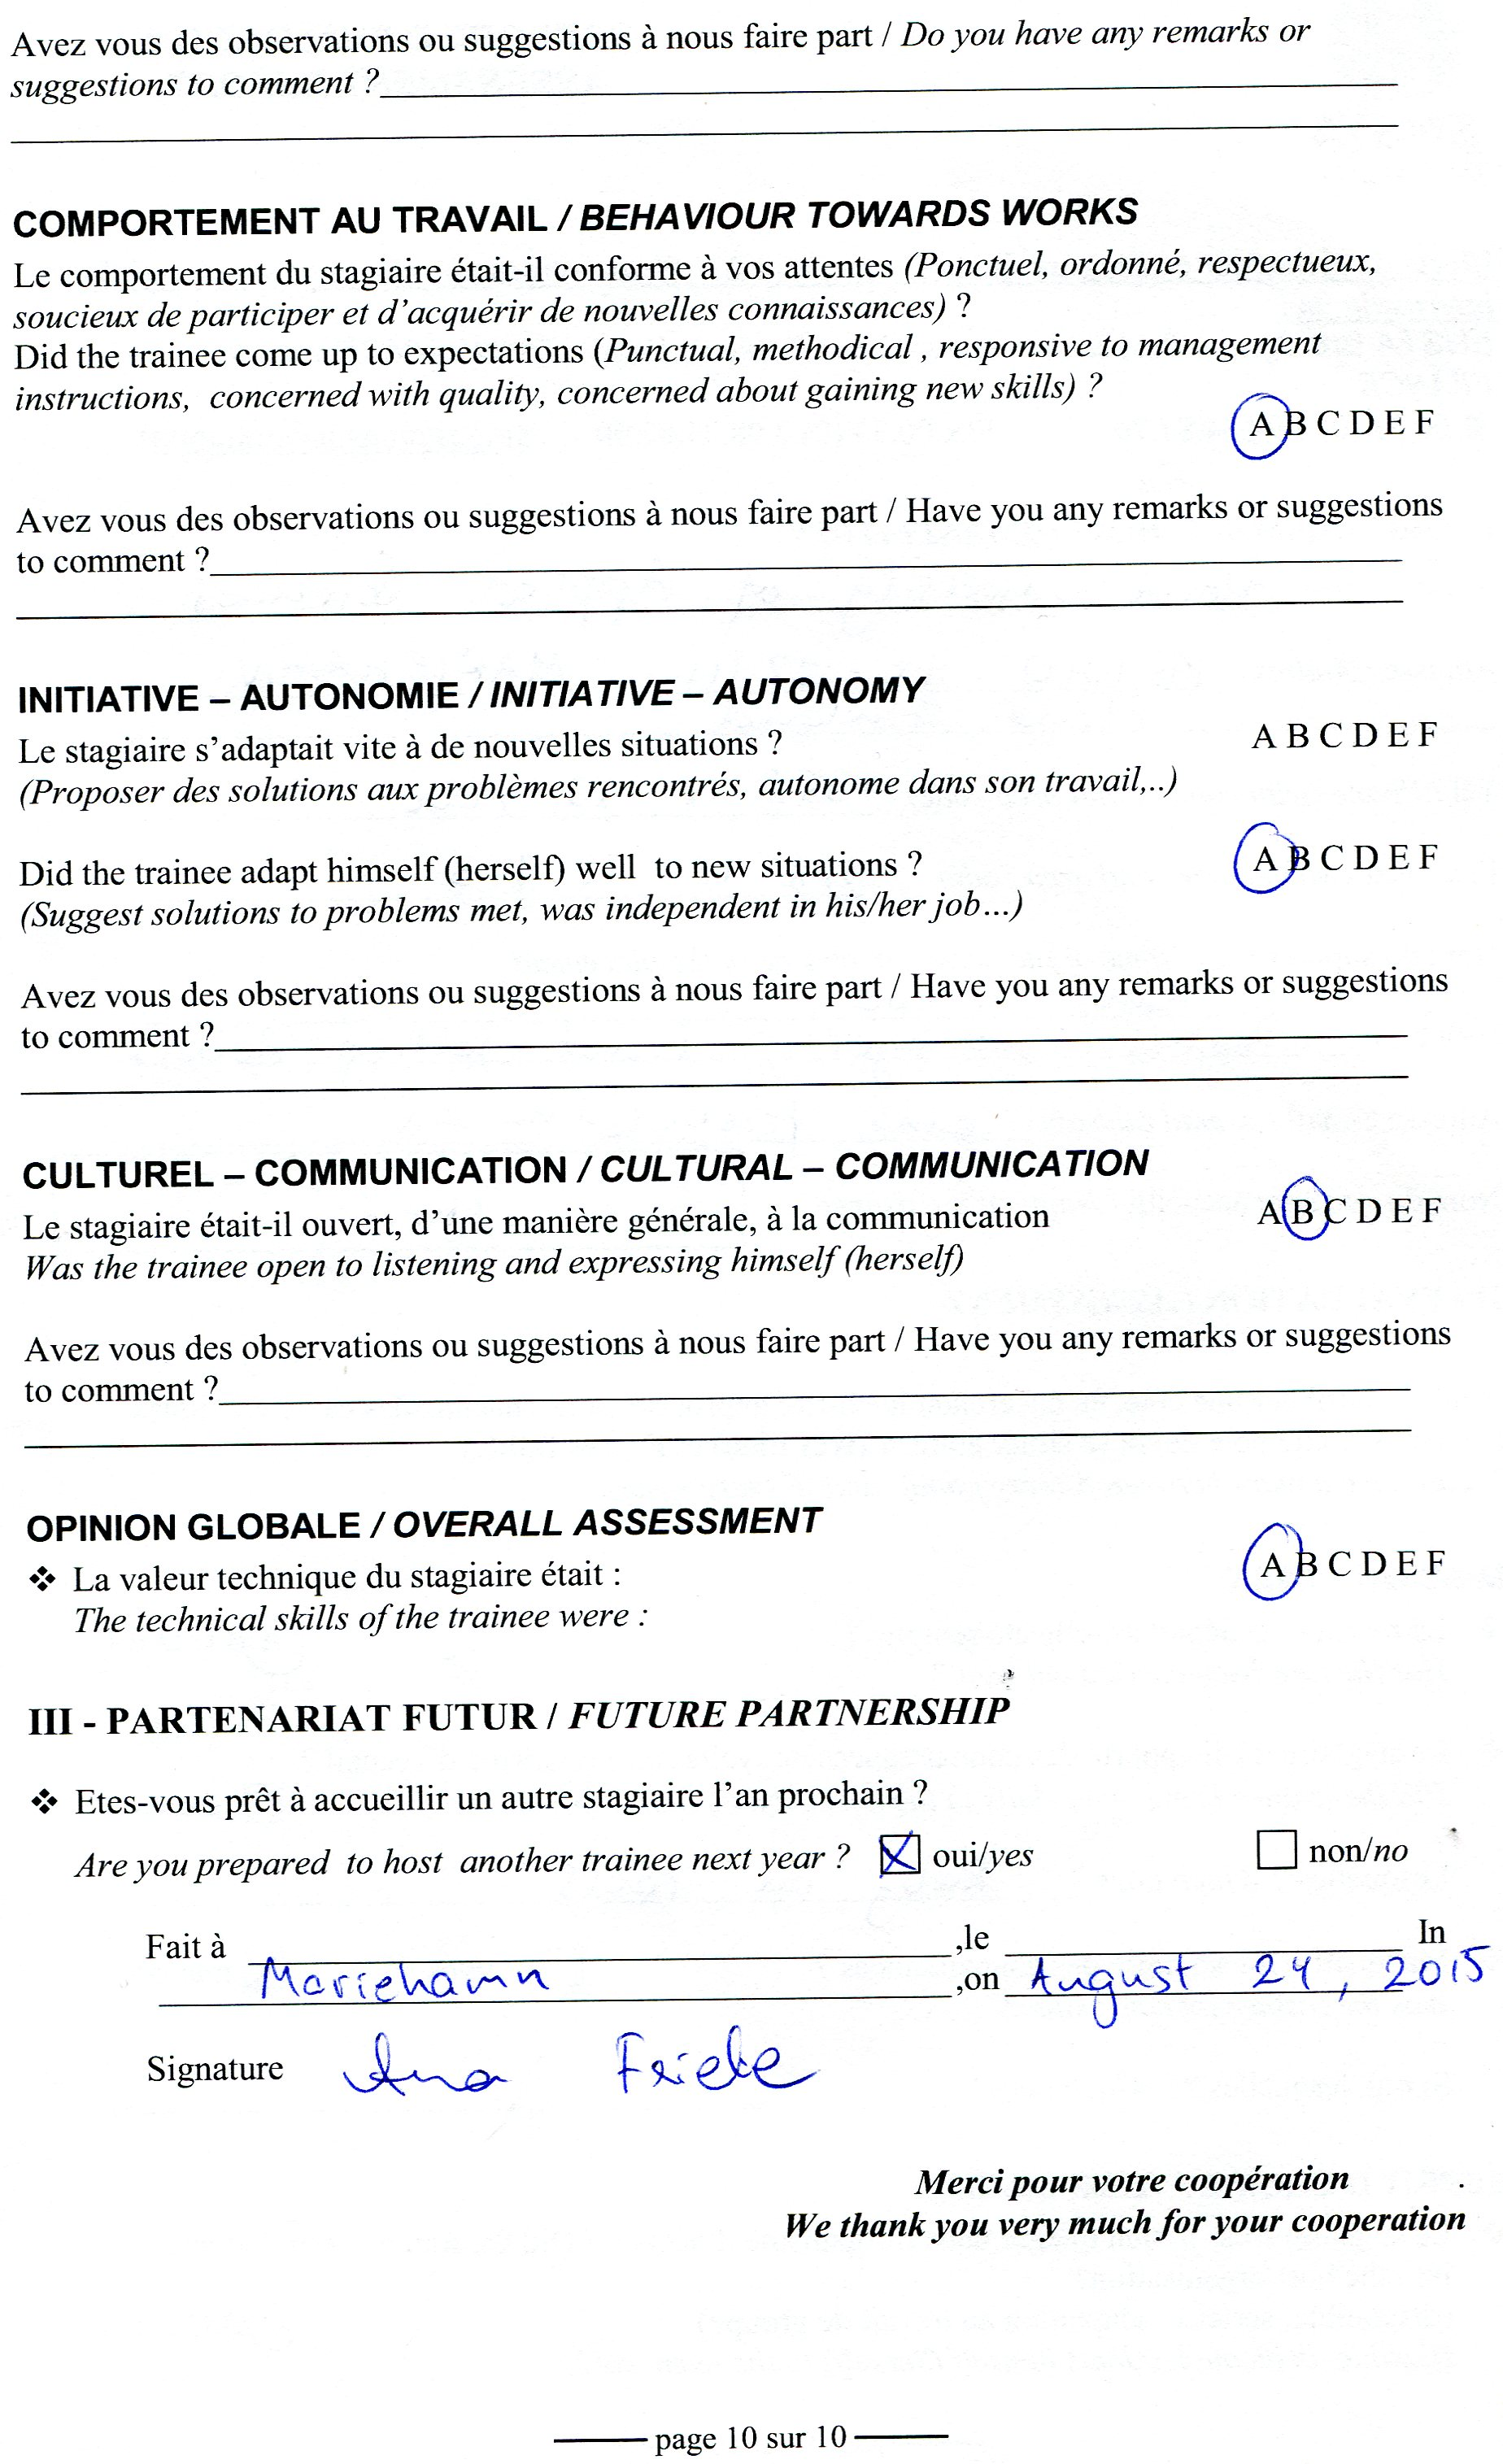
\includegraphics[width=12cm]{recto.jpg}
    \label{fig-sample}
\end{figure}

\end{document}

%%% Local Variables: 
%%% mode: latex
%%% TeX-master: t
%%% End: 
